\documentclass[border=11pt]{standalone}

\usepackage{tikz,enumitem}
\usetikzlibrary{arrows,automata,calc,positioning}

\tikzset{
    every edge/.style={
	draw=black,
	thick,
    },
    state/.style={
	anchor=center,
	circle,
	draw=black,
	thick,
	minimum height=2cm,
	inner sep=8pt,
	outer sep=2pt
    },
    stage/.style={
	anchor=center,
	rectangle,
	rounded corners,
	draw=black,
	thick,
	inner sep=8pt,
	outer sep=2pt
    },
}

\newcommand\stage[2]{%
    \parbox{3cm}{%
    \textbf{#1}\vspace{2pt}%
    \begin{itemize}[noitemsep,nosep,leftmargin=1.5em,labelsep=4pt]
    #2
    \end{itemize}}}


\begin{document}

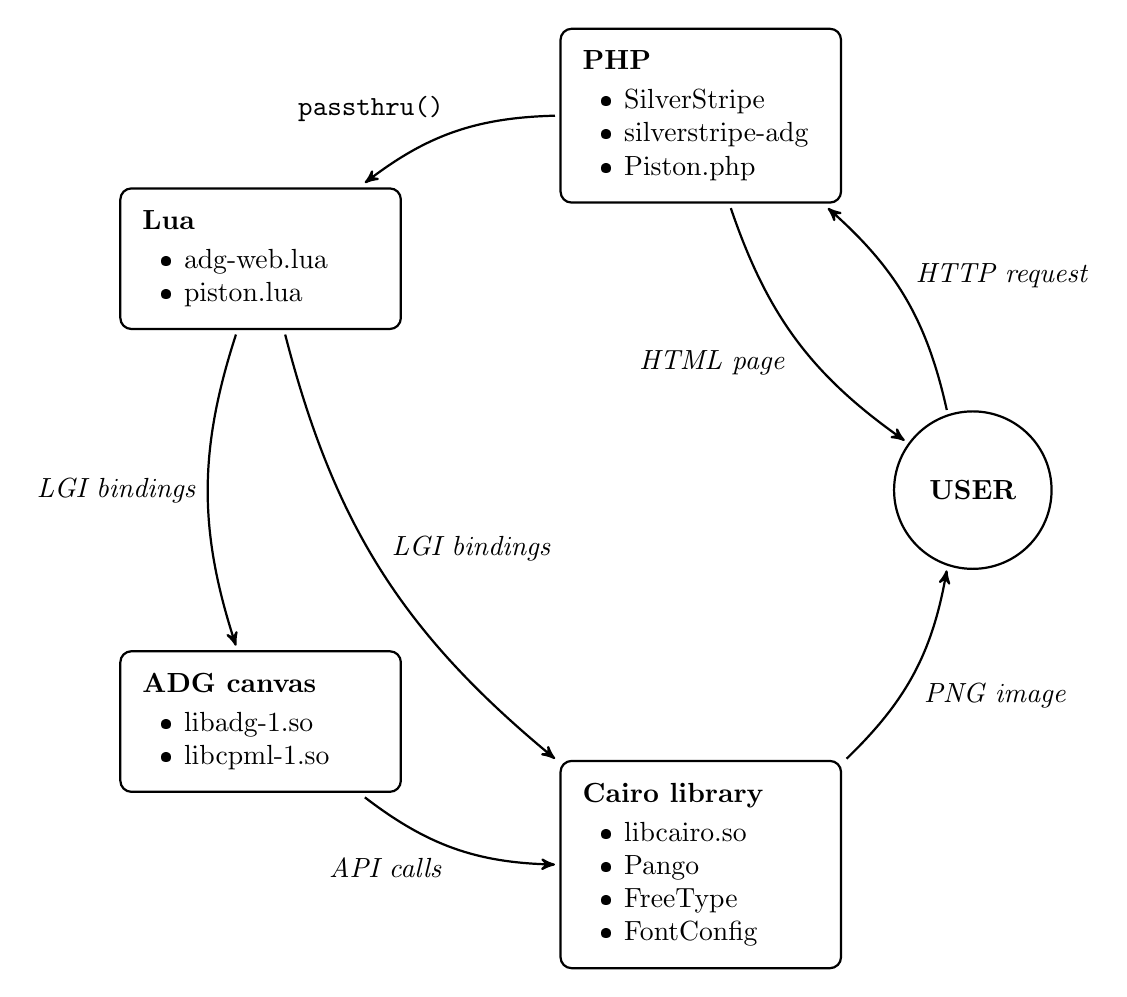
\begin{tikzpicture}[->,>=stealth']

    \node[state, minimum width=2cm, outer sep=2pt] (USER) at (0:5cm) {%
	\textbf{USER}};

    \node[stage] (PHP) at (72:5cm) {%
	\stage{PHP}{%
	    \item SilverStripe
	    \item silverstripe-adg
	    \item Piston.php}};

    \node[stage] (LUA) at (144:5cm) {%
	\stage{Lua}{%
	    \item adg-web.lua
	    \item piston.lua}};

    \node[stage] (ADG) at (216:5cm) {%
	\stage{ADG canvas}{%
	    \item libadg-1.so
	    \item libcpml-1.so}};

    \node[stage] (CAIRO) at (288:5cm) {%
	\stage{Cairo library}{%
	    \item libcairo.so
	    \item Pango
	    \item FreeType
	    \item FontConfig}};


    \path (USER)  edge[bend left=-18] node[above right]
	{\textit{HTTP request}} (PHP);
    \path (PHP)   edge[bend left=-18] node[above left]
	{\texttt{passthru()}} (LUA);
    \path (LUA)   edge[bend left=-18] node[left]
	{\textit{LGI bindings}} (ADG);
    \path (ADG)   edge[bend left=-18] node[below left]
	{\textit{API calls}} (CAIRO);
    \path (CAIRO) edge[bend left=-18] node[below right]
	{\textit{PNG image}} (USER);

    \path (PHP) edge[bend left=-18] node[below left]
	{\textit{HTML page}} (USER);
    \path (LUA) edge[bend left=-18]  node[above right]
	{\textit{LGI bindings}} (CAIRO);
\end{tikzpicture}
\end{document}

